

\subsection{Η άντληση πληροφορίων από την οπτικοποίηση}

Θα κάνουμε κάποια σχόλια πρώτα για το πως αναπτύχθηκε η οπτικοποίηση των δεδομένων και έπειτα
θα κάνουμε σχόλια για αποτελέσματα που φάνηκαν.
Επειδή ο αριθμός των σχεδιαγραμμάτων των δεδομένων είναι αρκετά μεγάλος, δεν θα τις προσθέσουμε σε αυτό το κεφάλαιο.

Η βασική συνάρτηση που βρίσκεται πίσω από την δημιουργία σχεδιαγραμμάτων των 
\texttt{timeSeries} του κάθε πειράματος,
είναι η \texttt{printDataBasedOnDate}.

Σε αντίθεση με ότι υπονοεί το όνομα της συνάρτησης για σχεδιασμό μέσω ημερομηνίας,
Η συνάρτηση αυτή σχεδιάζει τα \texttt{timeSeries} δεδομένα των πειραμάτων, ομαδοποιημένα με βάση
τις διακριτές τιμές οποιαδήποτε στήλη της \texttt{userInputData} επιθυμούμε  ,δίνοντας το αντίστοιχο όνομα της στήλης.

Όταν μιλάμε ομαδοποίηση με διακριτές τιμές, εννοούμε ότι βάζουμε σε μία κοινή ομάδα όσα 
πειράματα έχουν την ίδια τιμή για το πεδίο, για παράδειγμα όλα τα πειράματα που γίνουν στις
14 Οκτώβρη, και το κάνουμε αυτό για όλες τις τιμές της στήλης που μας δόθηκε που είναι ξεχωριστές.
Χρησιμοποιούμε τον όρο διακριτές και όχι ξεχωριστές, επειδή δεν είναι ότι έχουν κάποια ξεχωριστή 
ιδιότητα, αλλά ότι είναι διαφορετικές μεταξύ τους.

Αν τις δώσουμε πολλαπλά ονόματα στηλών της \texttt{userInputData},
θα ομαδοποιηθούν με σειρά αντίθετης της σειράς που τα εισήγαμε.
Δηλαδή, θα ξεκινήσουμε την επανάληψη ομαδοποιήσεων αλλάζοντας τις διακριτές τιμές τις τελευταίας στήλης,
δηλαδή της στήλης που δόθηκε πιο δεξιό στην λίστα ονομάτων που δώσαμε στις παραμέτρους της συνάρτησης,
κρατώντας τις άλλες στήλες σταθερές και βλέποντας ποια πειράματα υπάρχουν για αυτές τις διακριτές τιμές
των στηλών της \texttt{userInputData}
Αφού εξαντληθούν όλες οι διακριτές τιμές της τελευταίας στήλης,
θα αλλάξουμε την διακριτή τιμή της προτελευταίας στήλης, το όνομα που είναι δεύτερο πιο δεξιά, και θα επαναλάβουμε τις διακριτές τιμές της τελευταίας στήλης,
και πάει λέγοντας μέχρι να τελειώσουν οι διακριτές τιμές της προτελευταίας στήλης, όπου μετά πάμε στην αμέσως επόμενη διακριτή τιμή.
Όλο αυτό συνεχίζει μέχρι να δούμε όλες τις δυνατές ομαδοποιήσεις των στηλών που μας δόθηκαν.

Εδώ πρέπει να σημειώσουμε ότι στην υλοποίηση που πραγματοποιήσαμε, η ομαδοποίηση γίνεται εξωτερικά της συνάρτησης και παίρναμε σαν
παραμέτρους τις ομάδες που δημιουργήσαμε στην \texttt{printDataBasedOnDate},για την δημιουργία των σχεδιαγραμμάτων.
Η συνάρτηση δουλεύει με το να έχουμε την ομαδοποίηση από έξω από την συνάρτηση,
και να βάλουμε τα ονόματα μέσω στην συνάρτηση ομαδοποίησης, την \texttt{groupby()},
αλλά και μέσα στην αρχή της συνάρτησης ,παίρνοντας τα ονόματα σαν παράμετρο της συνάρτησης.
Θα διατηρηθεί η εξωτερική ομαδοποίηση επειδή με αυτήν έχουμε δουλέψει.

Ο λόγος που εστιάζουμε τόσο στην ομαδοποίηση με διακριτές τιμές είναι διότι αποτελεί ένα πολύ
δυνατό εργαλείο διαχείρισης των dataframes της pandas, 
την μέθοδο \texttt{groupby()},το οποίο χρησιμοποιούμε πολύ από εδώ και πέρα ,
για να διαχειριστούμε  κυρίως τα \texttt{timeSeries},αλλά και τα \texttt{userInputData}.

Δίνουμε επίσης και ονομαστικά τον τύπο της ομαδοποίησης που θα έχουμε, εκτός από την ομαδοποίηση με βάση τις θέσεις
των αισθητήρων που δηλώνει η στήλη \texttt{room},μέσω της  \texttt{\detokenize{type_of_other_grouping}},
δηλώνουμε λέξεις που δηλώνουν τον σκοπό της ομαδοποίησης βάση μίας στήλης ή πολλών στηλών.
Πέρα από την χρήση της μεταβλητής αυτής για παραπάνω νοηματοδότηση των ομαδοποιήσεων που θα πραγματοποιήσουμε,
την χρησιμοποιούμε και για να ενεργοποιήσουμε παραπάνω λειτουργικότητα στην συνάρτηση \texttt{printDataBasedOnDate}.

Η βασική χρήση της \texttt{\detokenize{type_of_other_grouping}} είναι το να περάσουμε μέσα του την λέξη \textbf{position},
όταν έχουμε τις παραμέτρους  \texttt{x axis} και \texttt{y axis}.
Όταν δίνουμε την νοηματοδότηση \textbf{position},σημαίνει ότι πάμε να δούμε την οπτικοποίηση των δεδομένων των πειραμάτων
για κάθε διακριτή θέση πηγής ρύπου, με όλες τις άλλες συνθήκες σταθερές.
Για αυτό και μπαίνουν πάντα τελευταία στις στήλες που ορίζουμε για ομαδοποίηση.

Όταν το κάνουμε αυτό, σε κάθε δημιουργία ομάδα σχεδιαγραμμάτων στην συνάρτηση \texttt{printDataBasedOnDate},έχουμε 
και το σχεδιάγραμμα με του δωματίου, που υποδεικνύει όλες τις θέσεις πηγών ρύπου που έχουμε ορίσει για την συγκεκριμένη δομή αισθητήρων,
αλλά και σε ποια θέση πηγή ρύπου είμαστε τώρα και τις ευκλείδειες αποστάσεις μεταξύ της συγκεκριμένης πηγή ρύπου και τους
αισθητήρες.

Κρατάμε σταθερά τα χαρακτηριστικά χρώματα που είχαμε για τους αντίστοιχους αισθητήρες και στην grafana, δηλαδή μπλε για το αισθητήρα
με id=0,πράσινο για id=1 και κίτρινο για id=2.Για κάθε πείραμα μέσα σε κάθε μία ομαδοποίηση, δίνουμε έναν υπότιτλο για τα διάφορα 
χαρακτηριστικά του.

Με την \texttt{printDataBasedOnDate} οπτικοποιούμε τα δεδομένα όλων των αισθητήρων για κάθε πείραμα στο ίδιο διάγραμμα.
Αλλά επειδή τα μηχανικά μοντέλα πραγματοποιούνται στο κάθε αισθητήρα ξεχωριστά, έχουμε ορίσει 
την συνάρτηση \texttt{plantDataGroupedByEuclidianDistance},η οποία οπτικοποιεί τα δεδομένα του αισθητήρα που δώσουμε
σαν παράμετρο στην συνάρτηση σε ξεχωριστό διάγραμμα το καθένα,
ταξινομημένα με βάση την ευκλείδεια απόσταση του αισθητήρα από την κάθε πηγή 
ρύπου και όχι από τον \texttt{x axis} και \texttt{y axis}.
Έτσι, είναι πολύ πιο εύκολα να δούμε πως η απόσταση επηρεάζει τα δεδομένα.

Τα σχόλια που έχουμε να παραθέσουμε είναι ότι τα εξής:

\begin{enumerate}
    \item Τα δεδομένα κυμαίνονται σε μια σχετικά μονοτονικά αυξητική συμπεριφορά ,δηλαδή μπορεί να φανεί ότι με τον χρόνο, η τιμή των VOC αρχίζει να αυξάνεται όσο υπάρχει η πηγή ρύπου στον χώρο, στην πλειοψηφία των πειραμάτων.
    \item Η περίοδος που εισερχόμαστε στον χώρο για να εισάγουμε την πηγή ρύπου, συνήθως μεταξύ στα 20 και 60-70 δευτερόλεπτα, υπάρχει μια παραπάνω αναταραχή των τιμών, που υποδεικνύει
    αντίδραση των αισθητήρων στο γεγονός που συμβαίνει.
    \item Οι αισθητήρες που η πηγή του ρύπου είναι πολύ κοντά, κάτω από μισό μέτρο δηλαδή, θα φτάσουν σε κάποια στιγμή που η τιμή τους θα φτάσει είτε στην μέγιστη δυνατή τιμή,
    τα 1000 ppm δηλαδή, είτε πολύ μεγαλύτερη από το συνηθισμένο, όπως τα 200 ppm.
    \item Δυστυχώς, και εδώ είναι το μεγάλο σημείο, δεν υπάρχει κοινή συμπεριφορά μεταξύ της πλειοψηφίας των πειραμάτων στην ίδια θέση πηγής ρύπου.
    Υπάρχουν μεγάλες διαφορές μεταξύ των πειραμάτων, οι αυξήσεις και μειώσεις κατά την διάρκεια του πειράματος είναι αταίριαστες μεταξύ των πειραμάτων.
    Ακόμα και στην πιο σταθερή περίπτωση που ο αισθητήρας είναι δίπλα από το πείραμα, δεν έχουμε κοινή συμπεριφορά.
    \item Με βάση προσπάθειας μελέτης των τοπικών ακροτάτων των δεδομένων, δεν καταφέραμε να εξάγουμε κάποια κοινή συμπεριφορά για τα δεδομένα.
    Ο κώδικας αυτός βρίσκεται στο notebook \texttt{find peaks},
    το οποίο όμως notebook έχει αναπτυχθεί παλιότερα και δεν έχει ανανεωθεί και ελεγχθεί για να συμφωνεί με μετέπειτα αλλαγές
    εκτέλεσης του κώδικα, όποτε δεν είναι σίγουρα ότι θα δουλέψει για τον χρήστη.
    \item Δεν εντοπίσαμε να υπάρχει συμπεριφορά καθυστέρησης αύξησης των δεδομένων όταν η πηγή ρύπου είναι κοντά, σε σχέση με όταν είναι μακριά.
\end{enumerate}

Οπότε, η εικόνα που μας δίνει η οπτικοποίηση δεν είναι καλή για την δυνατότητα των δεδομένων να εκπαιδεύσουν μηχανικό μοντέλο.
Για αυτό λογό προσπαθήσαμε να εκμεταλλευτούμε την συμπεριφορά που έχουν η αισθητήρες όταν η πηγή είναι πολύ κοντά.
Επίσης,δοκιμάσαμε  να επιλέξουμε υποκατηγορία των δεδομένων που μας φαίνονται πιο κοντά σε συμπεριφορά,
όπως και να ολισθήσουμε τα δεδομένα σε σημείο που θα περιμέναμε ιδεατά να βρούμε τα πειράματα να αυξάνονται τα VOC τους.

\begin{figure}[!htbp]
    \centering
    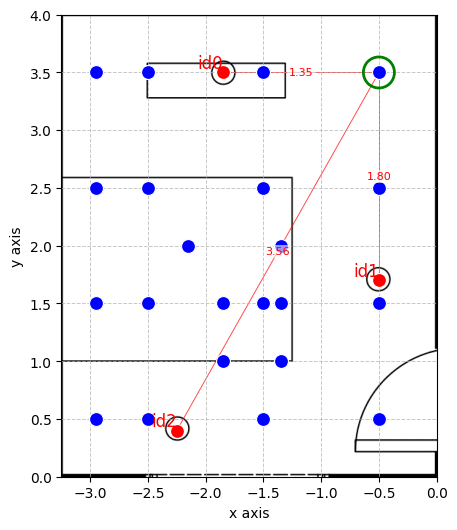
\includegraphics[height=6cm]{εικόνες/εικόνες σχετικά με την ανάλυση δεδομένων/παράδειγμα δωματίου.png}

    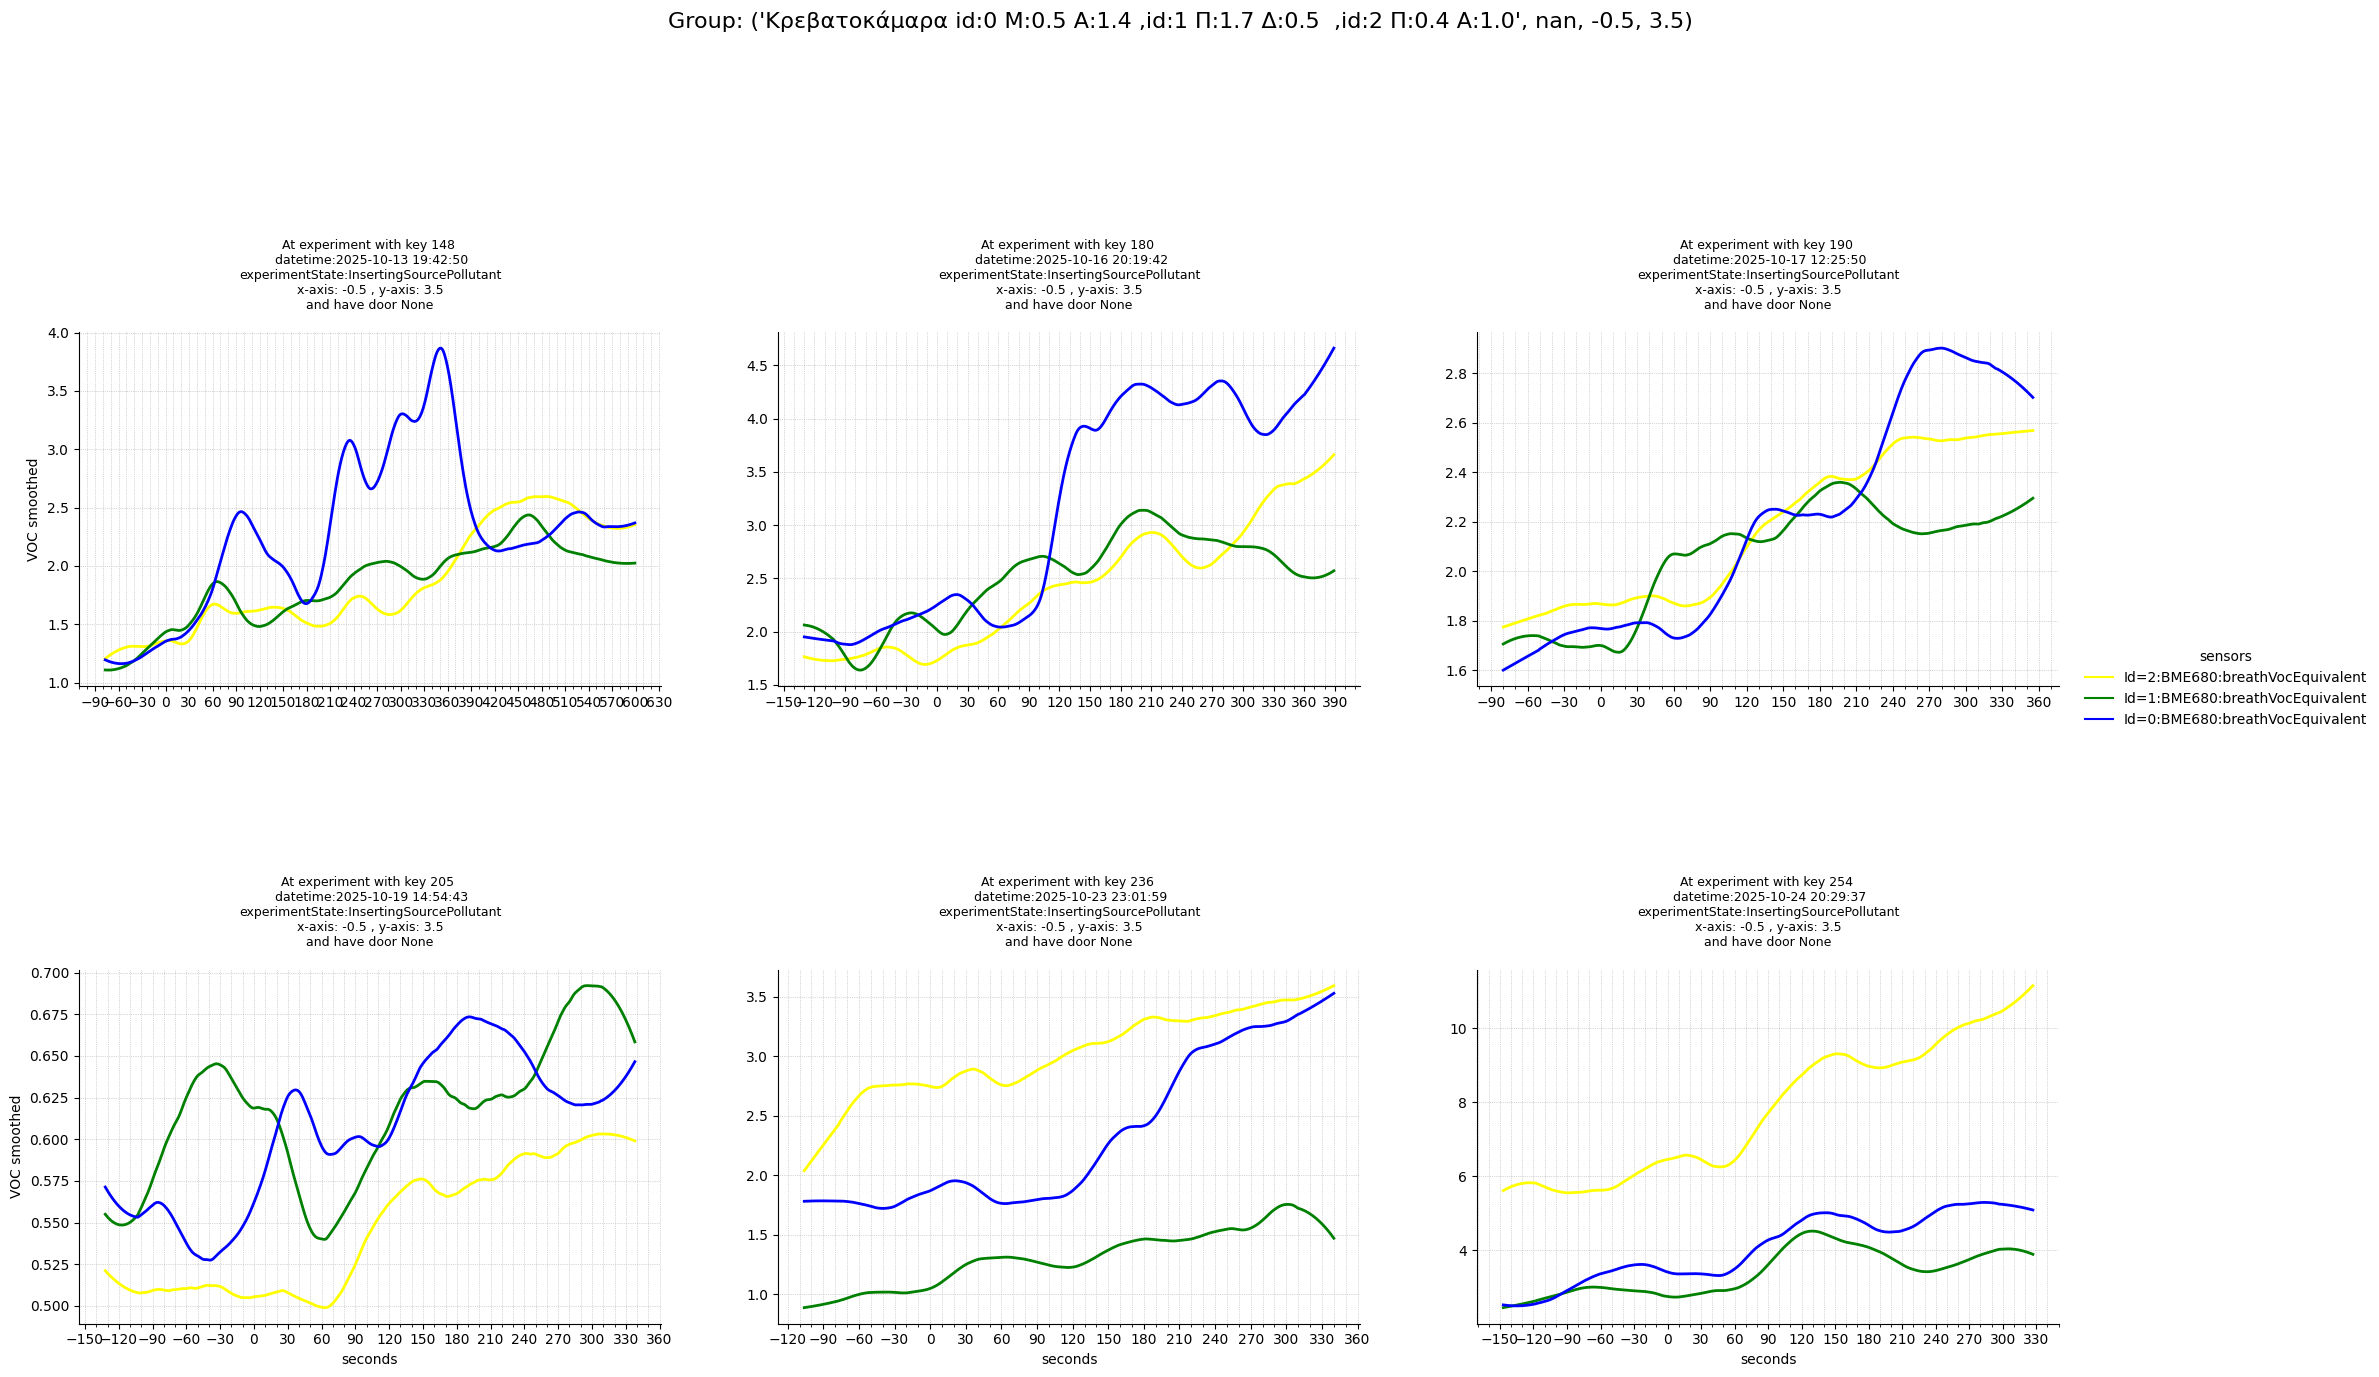
\includegraphics[height=10cm]{εικόνες/εικόνες σχετικά με την ανάλυση δεδομένων/παράδειγμα χρονοσειρών.png}

    \caption{Παράδειγμα των διαγραμμάτων δωματίου και χρονοσειρών που δημιουργείται από ομαδοποίηση βάση θέσης}
    \label{fig:timeseries}
\end{figure}